\documentclass[../../main.tex]{subfiles}
\graphicspath{{\subfix{../../image/}}} % 指定图片目录,后续可以直接使用图片文件名。

% 例如:
% \begin{figure}[H]
% \centering
% \includegraphics[scale=0.4]{图.png}
% \caption{}
% \label{figure:图}
% \end{figure}
% 注意:上述\label{}一定要放在\caption{}之后,否则引用图片序号会只会显示??.

\begin{document}

\section{主理想整环与唯一分解整环}

\begin{definition}[主理想整环]
设 $(R, +, \cdot)$ 是一个交换环,则我们称 $R$ 是个\textbf{主理想整环},若 $R$ 是一个整环,而且每一个理想 $I \lhd R$ 都是主理想,即存在$a\in \mathbb{R}$,使得
\begin{align*}
I = (a) = Ra
\end{align*}
的形式。
\end{definition}
\begin{remark}
由\refpro{proposition:生成的理想的集合表示}即可得到上述$I = (a) = Ra.$
\end{remark}

\begin{lemma}\label{lemma:整数环的每个加法子群都是nZ}
$(\mathbb{Z}, +, \cdot)$ 的每个加法子群都具有 $n\mathbb{Z}$ 的形式。
\end{lemma}
\begin{proof}
不妨令 $I < \mathbb{Z}$ 是加法子群。
假如 $I$ 只包含了 $0$ 一个元素,那么 $I = \{0\} = 0\mathbb{Z}$。
假设 $I$ 包含了 $0$ 以外的元素,那么根据逆元的封闭性,$I$ 一定包含了一个正整数,因此$I\cap \mathbb{N} _1\ne \varnothing $.根据自然数集的良序公理,我们可以取到最小的那个正整数,称其为 $n$,即$n=\min \left\{ I\cap \mathbb{N} _1 \right\}$.下面,我们只须证明
\begin{align*}
I = n\mathbb{Z}
\end{align*}
一方面,任取$n \in I$,则 $n$ 生成的(加法)子群为
\begin{align*}
\langle n\rangle =\left\{ \underset{k\text{个}}{\underbrace{n+n+\cdots +n}}:k\in \mathbb{Z} \right\} =\left\{ nk:k\in \mathbb{Z} \right\} =n\mathbb{Z} .
\end{align*}
于是由子群$I$对加法的封闭性可知
\begin{align*}
n\mathbb{Z} =\left\{ \underset{k\text{个}}{\underbrace{n+n+\cdots +n}}:k\in \mathbb{Z} \right\} \subset I.
\end{align*}
另一方面,假设存在 $I \setminus n\mathbb{Z}$ 的元素,我们任取 $m \in I \setminus n\mathbb{Z}$。则根据带余除法,我们有
\begin{align*}
m = nq + r
\end{align*}
其中 $1 \leqslant slant r \leqslant slant n - 1$。而$n(-q)\in n\mathbb{Z}\subset I$.
则根据子群的性质,
\begin{align*}
r = m - qn = m + n(-q) \in I
\end{align*}
而这与 $n$ 是 $I$ 最小的正整数的事实相矛盾。这就证明了这个引理.
\end{proof}

\begin{proposition}[整数环是主理想整环]\label{proposition:整数环是主理想整环}
$(\mathbb{Z}, +, \cdot)$ 是个主理想整环。
\end{proposition}
\begin{proof}
利用\reflem{lemma:整数环的每个加法子群都是nZ}即得结论.
\end{proof}

\begin{lemma}\label{lemma:域只有两个理想:零和自身}
若 $(R, +, \cdot)$ 是一个环,则 $R$ 是一个域当且仅当 $\{0\}$ 和 $R$ 是 $R$ 中唯二的理想 $(R \neq \{0\})$。
\end{lemma}
\begin{note}
这个引理表明:\textbf{域只有两个理想,即 零和自身}.
\end{note}
\begin{proof}
{\heiti 必要性:}假设 $R$ 是一个域,而 $I$ 是一个理想。假设 $I \neq \{0\}$,任取 $a \neq 0$。则存在 $b \in R$,使得
\begin{align*}
ab = 1
\end{align*}
因此
\begin{align*}
1 \in Ra \subset RI \subset I
\end{align*}
所以由\hyperref[lemma:理想是整个环的充要条件]{引理\ref{lemma:理想是整个环的充要条件}(2)}可知$I = R$。

{\heiti 充分性:}假设 $R$ 唯二的理想是零和整个环。令 $a \neq 0$,则$\{0\}$就是$R$的极大理想.于是由\refpro{proposition:素理想的充要条件}可知,$R/\{0\}$就是一个域.又因为$R/\{0\}=R+0=R$,所以$R$ 是一个域。
\end{proof}

\begin{proposition}[域是主理想整环]\label{proposition:域是主理想整环}
若 $(R, +, \cdot)$ 是一个域,则 $R$ 是一个主理想整环。
\end{proposition}
\begin{proof}
由\reflem{lemma:域只有两个理想:零和自身}可知$R$只有两个理想$0$和$R$.又由\refpro{proposition:生成的理想的集合表示}可知
\begin{align*}
{0}=0\cdot R=(0),\quad R=1\cdot R=(1),
\end{align*}
故$R$ 是一个主理想整环。
\end{proof}

\begin{proposition}[主理想整环中的素理想与极大理想等价]\label{proposition:主理想整环中的非零素理想与极大理想等价}
设 $(R, +, \cdot)$ 是一个主理想整环,$\mathfrak{p} \neq \{0\}$,则$\mathfrak{p} \lhd R$ 是一个素理想等价于 $\mathfrak{p}$ 是一个极大理想。
\end{proposition}
\begin{proof}
$\Leftarrow:$由\refpro{proposition:在交换环中,每一个极大理想都是素理想}立得.

$\Rightarrow:$
用反证法。假设 $\mathfrak{p}$ 是素理想,而不是极大理想,则存在 $I \lhd R$,使得 $\mathfrak{p} \subsetneq I \neq R$。

因为 $R$ 是主理想整环,我们记 $\mathfrak{p} = (p)$,$I = (a)$。则由于 $\mathfrak{p} \subset I$,我们有
\begin{align*}
p \in I = (a)=aR.
\end{align*}
故存在 $b \in R$,使得
\begin{align*}
p = ab
\end{align*}
显然,$b$ 不能是单位(即存在乘法逆元的元素),因为不然的话我们就可以写 $a = pb^{-1}\in (p)=\mathfrak{p}$,从而由$\mathfrak{p}\lhd R$可知$I=(a)=aR\in \mathfrak{p}$,进而 $\mathfrak{p} = I$,导致矛盾。因此,$b$ 没有乘法逆元。

另外,由于 $I$ 是真理想,故 $a$ 也不是单位——否则 $1=aa^{-1} \in (a)=I$,进而由\hyperref[lemma:理想是整个环的充要条件]{引理\ref{lemma:理想是整个环的充要条件}(2)}可知 $I=(a) = R$矛盾!

现在 $ab=p \in \mathfrak{p}$,则 $a \in \mathfrak{p}$ 或 $b \in \mathfrak{p}$。假如 $a \in \mathfrak{p} = (p)$,则存在$c\in R$,使得$a=pc=cp$.从而
\begin{align*}
p=ab=pcb\Rightarrow p(1-cb)=0.
\end{align*}
又因为$R$是整环,且由$\mathfrak{p}\ne\{0\}$可知$p\ne0$,所以
\begin{align*}
1-cb=0\Rightarrow 1=cb=bc.
\end{align*}
故$b$ 就是一个单位,而这是不可能的。
假如 $b \in \mathfrak{p}$,则同理,$a$ 就是一个单位,而这也是不可能的。无论如何,我们都会得到矛盾。

因此,我们就证明了,在主理想整环中,每一个素理想都是极大理想,因此两个概念在主理想整环中是等价的。 
\end{proof}

\begin{figure}[H]
\centering
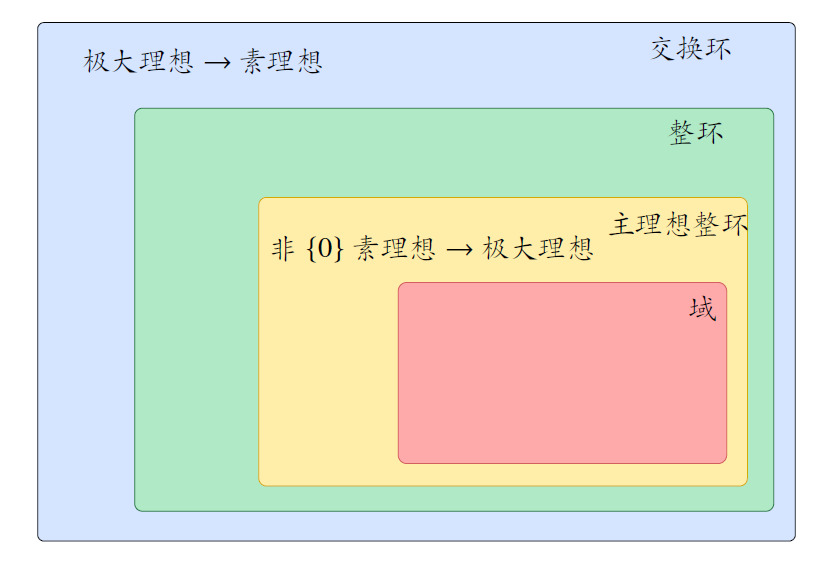
\includegraphics[scale=0.4]{环的层级关系以及素理想和极大理想之间的关系.png}
\caption{环的层级关系以及素理想和极大理想之间的关系}
\label{figure:环的层级关系以及素理想和极大理想之间的关系}
\end{figure}

\begin{proposition}\label{proposition:pZ是Z的一个域}
若 $p$ 是一个素数,则 $\mathbb{Z}_p$ 是一个域。
\end{proposition}
\begin{proof}
由\refpro{proposition:整数环中的素理想}可知$p\mathbb{Z}$就是$\mathbb{Z}$的素理想.再由\refpro{proposition:主理想整环中的非零素理想与极大理想等价}可知$p\mathbb{Z}$也是$\mathbb{Z}$的极大理想.于是由\refpro{proposition:极大理想的充要条件}可知$\mathbb{Z}/p\mathbb{Z}=\mathbb{Z}_p$是一个域.
\end{proof}

\begin{definition}
若 $p$ 是一个素数,则我们把 $\mathbb{Z}_p$ 记作 $\mathbb{F}_p$。特别地,又由$\mathbb{Z}_p=\{k+p\mathbb{Z},k=1,2,\cdots,p-1\}$可知,$\mathbb{Z}_p$是一个只有$p$个元素的有限域,即只有有限多个元素($p$个元素)的域.
\end{definition}

\begin{lemma}
若 $n$ 是一个合数,则 $\mathbb{Z}_n$ 既不是一个域,也不是整环.
\end{lemma}
\begin{proof}
先证$\mathbb{Z}_n$ 不是一个域.
由 \(n\) 是合数可知 \(n\) 不是素数, 从而由\refpro{proposition:整数环中的素理想}可知 \(n\mathbb{Z}\) 不是素理想.
又因为 \(\mathbb{Z}\) 是主理想整环, 所以由\refpro{proposition:主理想整环中的非零素理想与极大理想等价}可知 \(n\mathbb{Z}\) 不是极大理想.
故由\refpro{proposition:极大理想的充要条件}可知 \(\mathbb{Z}_n = \mathbb{Z}/n\mathbb{Z}\) 不是域.

再证$\mathbb{Z}_n$ 不是整环.
由 \(n\) 是合数可知, 存在 \(a, b \in \mathbb{Z}\) 且 \(a, b \ne \pm 1\), 使得 \(n = ab\). 从而 \(|a|, |b| < n\), 于是
\begin{align*}
\overline{a}\,\overline{b} = \overline{0}, \quad \text{且} \quad \overline{a} \ne \overline{0}, \overline{b} \ne \overline{0}.
\end{align*}
故 \(\mathbb{Z}_n\) 不是整环.
\end{proof}





\end{document}